\chapter{Воскресенка и озеро Радунка}

Южнее проспекта Ватутина – жилые массивы Радужный и Воскресенский, разделенные на пронумерованные микрорайоны. Жилмассив Радужный вытянулся через дорогу вдоль берега озера Радунки.

Сводка названий озера по имеющимся у меня картам – на плане участка Днепра в районе Киева, 1910 года: «оз. Радунка», на плане 1912 года опять «оз. Радунка», карта лоций 1914 года: «оз. Фроловское (Радунка)», советский план 1943: «оз. Радуга», немецкий план 1943: «Raduga – See», 1978: «оз. Радуга», 1979, 1981 – то же, 1991: «оз. Радунка (Радуга)». На картах 21 века его обозначают как «Радужное», «Радуга», «Радунка».

Очевидно, что Радунка – самое старое, а значит и верное название.

Озеро выглядит таким же отрезком луговой реки, как Гнилуша или Западный Залив, только помощнее, и восточным берегом примыкает к возвышенности, известной как левобережная Лысая гора. Оно длинное – 1,3 километра, и широкое, в среднем около 100 метров, причем это естественная ширина. Его долго обходить пешком. Летом берега облеплены людьми, днем они лежат, едят и купаются, а ночью пьют спиртные напитки, едят и тоже купаются. 

На южном берегу, там где частный сектор по улице Марка Черемшины – остатки Воскресенской слободки, причем остатки второй половины 20 века. Основная, старинная часть слободки была вдоль восточного берега, где с конца 1970-х стоят высотки.

Западный берег застроен дачным посёлком Воскресенские сады. На плане РККА 1930-х их нет в помине, однако мне нравится этот план своей ясностью:

\begin{center}
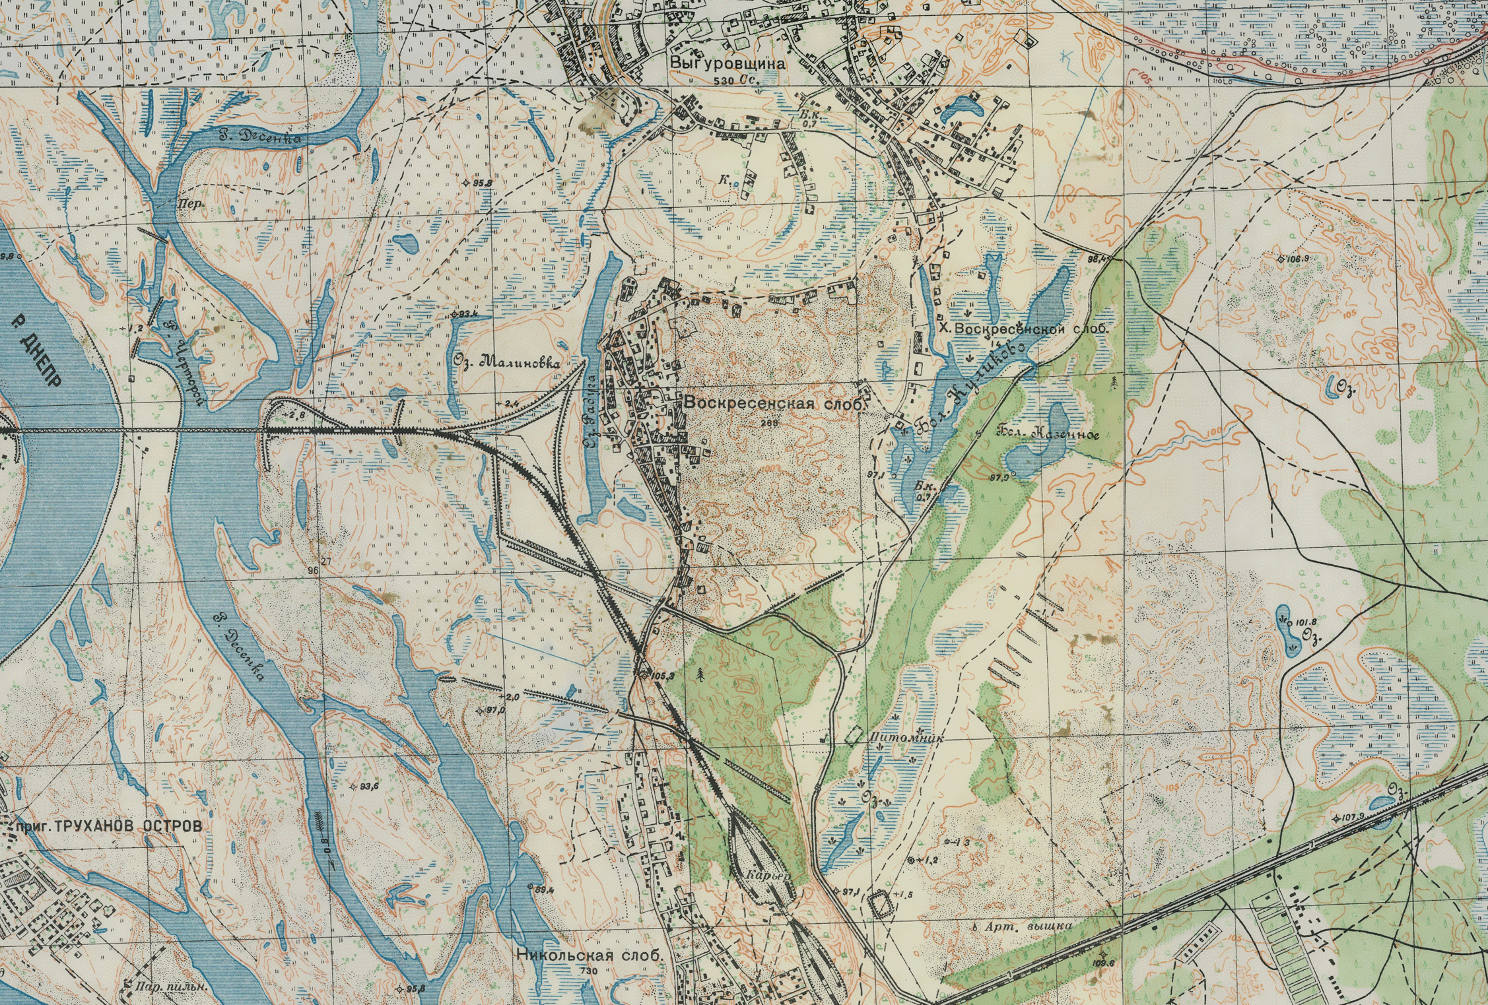
\includegraphics[width=\linewidth]{chast-gorodki/radujnoe/rkka-voskr-s.jpg}
\end{center}

Обратите внимание – там где не разлиты воды-болота, там непременно возвышенности, левобережные холмы.

Хороший ориентир, чтобы связать прошлое и настоящее – линия железной дороги от Петровского железнодорожного моста, идет таким черно-белым жирным пунктиром. Сейчас по левую сторону от нее, то бишь на запад и юг от нее – Русановские сады. А выше – Воскресенские.

Среди последних, за линией скоростного трамвая, параллельно озеру Радунке – озеро Малиновка, бывшая «речка Меленовка» из старинных земельных документов. От озера Радунки к Малиновке когда-то протекал канал, затем прокопанный дальше до водоема Неводного.

%Озеро Радунка еще относительно недавно было похоже на отрезок равнинной реки, чем и является, прежде будучи частью речки Радунки, на что красноречиво указывает название.

%Малиновка – рукав речки Радунки. Севернее Воскресенской слободки Радунка разделялась на два рукава. Один, восточный – известный ныне как озеро Радунка, протекал ближе к Воскресенке, а западный, ныне озеро Малиновка, слыл речкой Меленовкой.

Очевидна связь Меленовки с островом Меленовским, проходящим в земельных документах 17 века.

5 июля 1656 года он достался в качестве залога супругам Андрею Биримовичу (переяславскому войту) и Огрефине Огризковне Биримовичовой от инокини Печерского монастыря Марты, в миру Марыны Ходычанки, в первом супружестве жены Михаила Балыка, и сына супругов, Мартина Михайловича Балыка. Остров этот Михаил Балык получил от панов Ленкевичей, поэтому в бумагах часто упоминается как «остров Меленевский Ленковщина»\cite{mihdocs}:

\begin{quotation}
то ест остров, названый Меленевский, за рекою Днепром от миста Киева сугран села Милославсчыны, названое Викгуровсчызны и кгрунту воскресенском и николисского од урожоных пнов Алексанра Ленкевича и Погорского, подвоеводего и писара земского мозырского, и синовцов его, панов Ерого Казимера и Романа Ленковичов и Погорских
\end{quotation}

и есть такое уточнение:

\begin{quotation}
тот остров Меленевский Ленковсчизну, ту ж, под Киевом, за Днепром и рекою Чарториею лежачый,
\end{quotation}

Остров, конечно, был не сам по себе, а

\begin{quotation}
зо всими его пожитками, повинностями и приналежностями, кгрунтами, полями, сеножатми, розробками, дубровами, озерами и зо всими ин енере менеными и не менеными пожитками и прыналежностями
\end{quotation}

В выписи из «книг миских права майдеборского ратуша киевского» за 22 генваря 1670 года речь идет о продаже Григорием Биримовичем трети Ленковского хутора войту киевскому Данилу Полоцкому\cite{mihdocs}:

\begin{quotation}
футор, прозываемый Ленковский, правом заставным и отцу его и ему служачий за рекою Днепром от места Киева з границ села Викгуровщины лежачий, яко о всих границ певном и досконалом положеню и оцерклиованю футора того Ленковского, бору, лесков, прилузок, заков, поля, сеножатей и озер так грамота его царского пресвитлого величества на тот же футор небожчику еще пну Андрию Биримовичу, войту переяславскому
\end{quotation}

Остров Меленовский, он же Ленковский, да хутор Ленковский на нем.

5 августа 1693 года киевская мещанка Мария Полоцковна, Луцковичова в первом замужестве, Рызина во втором, дочь Данилы Полоцкого, завещает во владение игумену Михайловского Златоверхого монастыря Сильвестру Головчину и «всей капитуле Михайловской» ту же треть хутора Ленковского\cite{mihdocs}: 

\begin{quotation}
и поссессии своей третюю часть футора, называемого Ленковичовского, за рекою Днепром близко села Выкгуровщини певным граныц оцирклованем лежачую
\end{quotation}

Фамилия Рызина всплывает также в названии хутора, а на 1914 год уже просто урочища Ризавщины, что лежало между озерами Радункой и Малиновкой – теперь там дачные участки Воскресенских садов.

Что до острова Меленовского, вероятно так называлась суша между Малиновкой и Черторыей. На лоции 1914-го это «Михайловский луг», что логично, ибо остров достался Михайловскому монастырю. Небось луг прежде обозначался как Михайловский остров. Немецкий план 1943 года называет луг Михайловский уже одноименным болотом.

К северо-западу от Малиновки, параллельно ей и озеру Радунке, было озеро Неводное, на карте 1912 года соединенное с Малиновкой.%, а на плане Сноевского выведенное как самый западный рукав речки Гнилуши, что не совсем верно.

Неводное более не существует. До скачка с левого берега на остров Муромец, Московский мост начинается на большом полуострове, по коему идет проспект Генерала Ватутина. По картам прослеживается, что этот полуостров раньше был островом, омываемым Черторыей. Западный ее рукав ныне сохранился, примыкая к острову Муромцу. А восточный рукав, некогда основное, прямое русло, отсекал остров от материка со стороны Выгуровщины. Отмирая, рукав этот и стал озером Неводным\footnote{На 1943 год, исток: 50°29'50.45"N 30°33'53.64"E, устье: 50°29'12.88"N  30°33'43.7"E}. 

Сейчас на его месте – раздувшийся, безобразный залив Десенка – его видишь, когда перебираешься через Московский мост с Петровки. Справа, за Skymall и «Ашаном», и прячется этот залив. Другой стороной он примыкает к Воскресенским садам и загаженным верболозным пустырям за водоочистными сооружениями.

Но были и другие изменения местности. Кроме прочего – сооружение дамбы, которая продолжается железнодорожным мостом Петровского. Дамба перерезала многие водотоки. Приложила руку и разрушающая всё на пути своем Черторыя. Старое русло ее, ставшее озером Неводным, продолжалось южнее, параллельно нынешнему руслу Черторыи. Это продолжение осталось в виде озера Русановского на Русановских садах.

Прежде чем мы отправимся туда, закрепим.

В некотором прошлом, на широте Московского и Петровского мостов, у Черторыи было два рукава. В западный влился Днепр и надул рукав до ширины Днепра. Восточный же остался не у дел и превратился в озера Неводное и Русановское.
  
Есть такие Русановские сады – дачные участки, протянувшиеся от Воскресенских садов на юг к Никольской слободке. Улицы носят одинаковое название – Садовая, отличаясь номером от 1 до 32, и посередке идет Центральная Садовая. Вместо дач кое-где уже многоэтажные особняки.

В советское время туда добирались автобусом от метро Левобережки, или пешком, ибо автобусы ходили только в определенное время дня, уж не помню когда.

Сады опоясывает железная дорога, идущая по дамбе к Петровскому железнодорожному мосту. Примыкающая к ней северная часть Садов на карте лоций 1914 года обозначена как «урочище Боярское». Вероятно оно, как и поселок Боярка, изначально принадлежало каким-то боярам.

Между дачами и Черторыей – луговая, заросшая вербами местность Горбачиха. Название Горбачихи на нем\-ецком плане 1943 года – болото Кодачок.

%Сопоставлять ее с чем-то древним язык не поворачивается. Еще в середине 19 века там были часть восточного берега Труханова острова, русло Черторыи и остров, исчезнувший ныне кроме южной половины, что теперь стала северной частью острова Кута («угла») (сейчас это считается северной половиной острова Долобецкого, хотя последний, южный, поныне отделен от Кута проливом). 

У меня есть только два плана с названиями здешних урочищ более подробными, нежели на остальных картах. Это карта лоций 1914 года и немецкая 1943 года. На первой озеро Малиновка подписано южнее той длинной прямой Малиновки, что видна на картах уже несколько веков. 

Хорошо, допустим, подписали низовье Малиновки, которое отрезано железной дорогой и находится сейчас в Русановских садах. Однако на карте лоций есть урочище Боярское на запад от «оз. Малиновка», примерно где 28-24 Садовые улицы. Это от железной дороги на юг. А карта 1943 года показывает болото Боярское севернее железной дороги, хотя и тоже – западнее Малиновки, но уже «традиционной», которая параллельна озеру Радунке.

Логически можно выстроить соображение, что давнее Боярское урочище лежало к западу от давней «речки Меленовки», еще не перерубленной железной дорогой. Поэтому справедливо считалось и болото Боярским, как часть большего урочища. Либо на картах что-то напутано.

По Горбачихе тоже проложена дамба, противопаводковая, а теперь еще и Подольско-Воскресенский мост. И между дамбами и основной частью садов изогнулось змеей озеро Русановское. Раньше на юге оно соединялось с Черторыей, да было перегорожено дамбой.

На западном берегу южной части озера, примерно до конца 20 века существовало две базы отдыха – домики на сваях. Одна база – от Академии Наук, наша семья там отдыхала, хотя к Академии Наук отношения не имела. К воротам вела, кажется, 16-я Садовая улица. Добирались к ней сначала по Центральной Садовой, потом сворачивали да шли ровной грунтовкой. Справа открывались озерца между участками. Темные, тихие воды, где плавно передвигались улитки.

Идешь себе, минуешь бетонный мостик, снова прямо, потом через лежащую поперек Прибрежную улицу, к важным, кованным воротам, увитым хмелем и диким виноградом. За оградой – комариные домики, дорожки из бетонных плит, высокие тополя, душевые, два туалета, стеклянная столовка и – административный корпус в настоящей барже.

В начале девяностых меня это не озадачивало. Потом стало. Я не понимал, как в озеро попала баржа. И лишь теперь стало ясно – ее ввели в Русановское озеро из Черторыи, когда еще не было дамбы. Потом дамба замкнула выход и русло оказалось отрезанным от Черторыи. Отмечу, что дачники Русановских садов вместо Черторыи говорят Десенка.

Мы плавали по озеру на качавшемся у берега ржавом понтоне. Кажется еще на чем-то. И я лазал просто вдоль берега, мимо дач, хозяева коих укрепляли свои участки от размыва заборами, спинками пружинных кроватей и прочим мотлохом.

Весной 2013 года я отправился на велике искать эту базу отдыха. Не был там с девяностых, знал, что после Академии Наук ее вроде выкупила некая религиозная община – либо это относилось к соседней базе, не знаю. Хотелось поглядеть, что осталось.

Снег еще толком не сошел, повсюду были лужи – одни ледяные, другие уже растаявшие и мутные. Дачники жгли мусор, пахло дымом. Я перетащил велик через рельсы на высокой насыпи, спустился с пустой железнодорожной платформы по крутой лестнице, закрутил педали. Сворачивал наобум. Сыро, мрачно, не как прежде.

А было лето, солнечно, и мы ходили на пляж за дамбой, там вообще-то два пляжа, один за Третьей Дамбовой улицей, другой, с разрушенным причалом – около Девятой Садовой, но мы шли на первый, поближе. Я переплывал через Десёнку на Долобецкий остров, не зная его имени, грелся там на берегу, и плыл назад. Мне было лет 16-17. Мы отдыхали на Русановских садах несколько лет.

Память подсовывает куски того времени. Вот мы с бабушкой Таней быстро шагаем по Центральной Садовой – автобус днем не ходил. А вот я еду к бабушке на Лукьяшу, играю там на братовой «Денди» и прохожу бродилку «Нимо» – ох и сложно, особенно последний босс! Потом приезжаю к брату в Сады и хвастаюсь, что прошел игру.

А у бабушки тогда был телевизор, взятый напрокат – маленький, кажется «Юность», и пункт проката работал на улице Маршала Рыбалко, там бабушка купила нам с братом по дешевке списанные магнитофоны, я свой использовал для звукозаписи совместно с основным моим «Радиотехникой», подаренным отцом ко дню рождения. Черным вечером, когда сыпал снег, я поднимался улицей Коперника, фонари светили желтым, было хорошо.

Русановские сады давали странное ощущение, что ты находишься вне города посреди города. Видно правый берег, тогда еще без уродливых зданий, а так – золотые купола среди зелени, монумент Родины-Матери, чашу Вечного огня. За ними, на Бастионной, был мой дом.

Я не досиживал до конца смены отдыха – но оставались тётя, мой двоюродный брат и бабушка. А я посещал их уже наездами, на полдня, вот так было удобнее. Чем дышать в полутемном домике бальзамом «Гвоздика» да ходить в мрачный туалет или кормиться в столовой.

В столовке не кормили ничем особенным. Это не дом отдыха «Кротенки» под Полтавой, где семилетний я, преодолевая стеснение, ходил к поварам за добавкой огромных блинов на дрожжах. Эти блины, а вернее жареные круглые пирожки, подавались с вишневым вареньем. Макаешь и кусаешь.

Бетонные плиты, бадминтон под тополями. Лавка-качели возле ивы на берегу озера. А меж двумя деревьями, в плоть их, был вставлен турник. Я выкрутил его и бросил в воду. 

На барже завели видеотеку. О видеотеках – отдельная глава этой книги, здесь не буду. Комната с нею перекошена, как вся баржа, и у стен прибились мягкие, пыльные кресла. Сидя в таком, ноги оказывались почти вровень с головой из-за наклонности пола.

Чтобы попасть к пляжу, мы выходили на улицу, шагали мимо второй базы отдыха (у них не было своей столовки и своей баржи, готовили на газе из баллонов), затем поворачивали к пустырю около Русановского озера, с лавками-качелями, поднимались на дамбу, а чуть дальше спускались с нее через верболозы уже к пляжу. 

После плавания мне всегда становилось холодно, и я бродил по этим верболозам, пескам Горбачихи, грелся. Иногда мы с братом шли на север вдоль берега, шли, шли, шли, пока не надоедало. Там всё продолжался берег, но как-то добрались к заливчику, где в прозрачной воде вились пиявки.

Вместо денег в ходу были «купоно-карбованцы», и книжка в мягкой обложке по программированию на Turbo Pascal стоила 50000 этих купонов. Программами обменивались на дискетах 5,25 и 3,5 дюйма (емкостью 720 килобайт и 1,4 мегабайта). 

1994 год! В Киеве впервые проходит компьютерная выставка. Я пишу картины маслом. Дарю брату свой складной велосипед «Минск», а он мне – мой же скэйт, отданный ему раньше. Еще недавно, шестого мая, на день рождения, мама подарила мне две велосипедные камеры – в то время это был дефицит. Я поставил камеры, выехал во двор, а велик оказался мне уже маленьким, неудобным. Со мной лет с восьми, подкручивался по росту, и наконец – предел.

И вот 2013-й. Сворачиваю в «линии», ищу базу Академии Наук. Не то. Не тот путь. Не узнаю. Большие дома. Нет прежнего ориентира – единственного на весь поселок магазина «Меркурий». Выезжаю несколько раз к оплывшему белым льдом Русановскому озеру. 

Наконец вижу узнаваемый бетонный мостик через озерцо. Прямо. 

Упираюсь в ворота базы. Там закрыто, чужое, там спилены тополя, штабелями лежит металлические рейки, домики приспособлены под строителей Воскресенского моста, он почти дополз сюда, разрушая прошлое.

\newpage

\begin{center}
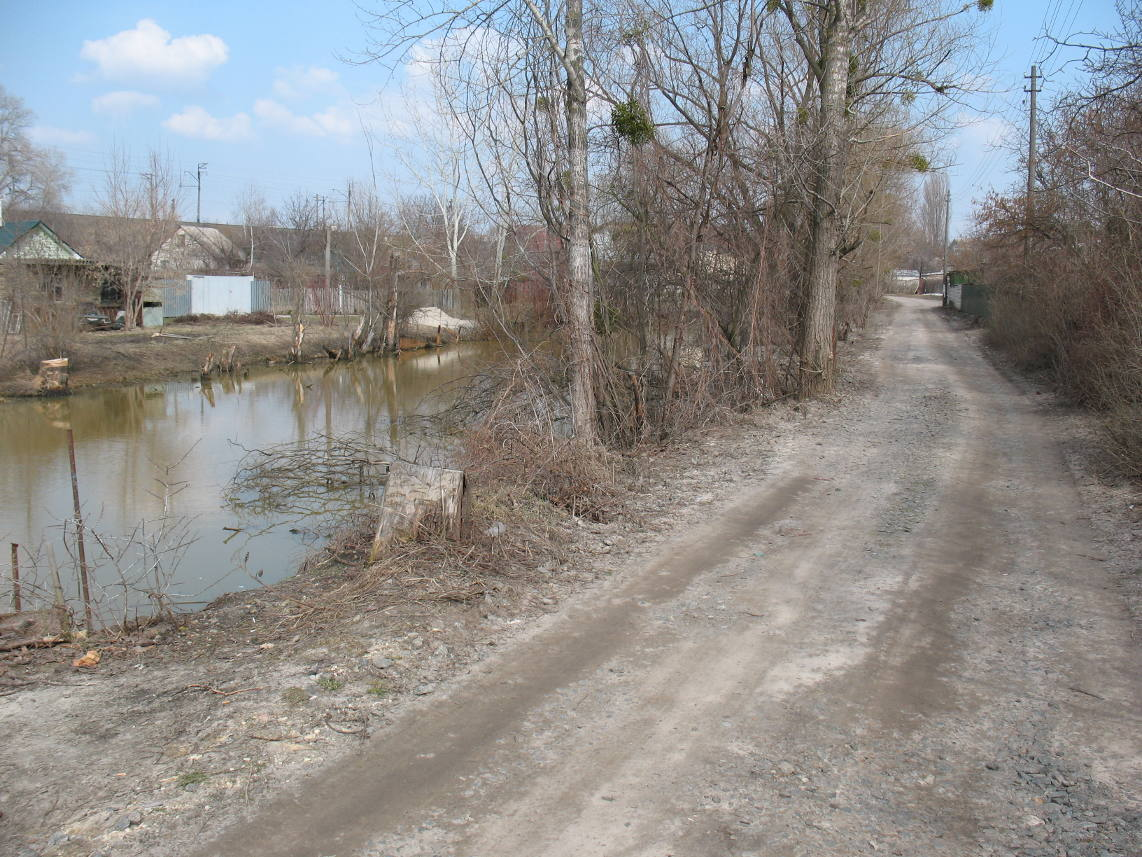
\includegraphics[width=0.98\linewidth]{chast-gorodki/radujnoe/s_IMG_2489.JPG}

\textit{2013 г. Русановское озеро около ж.д. дамбы.}
\end{center}

\begin{center}
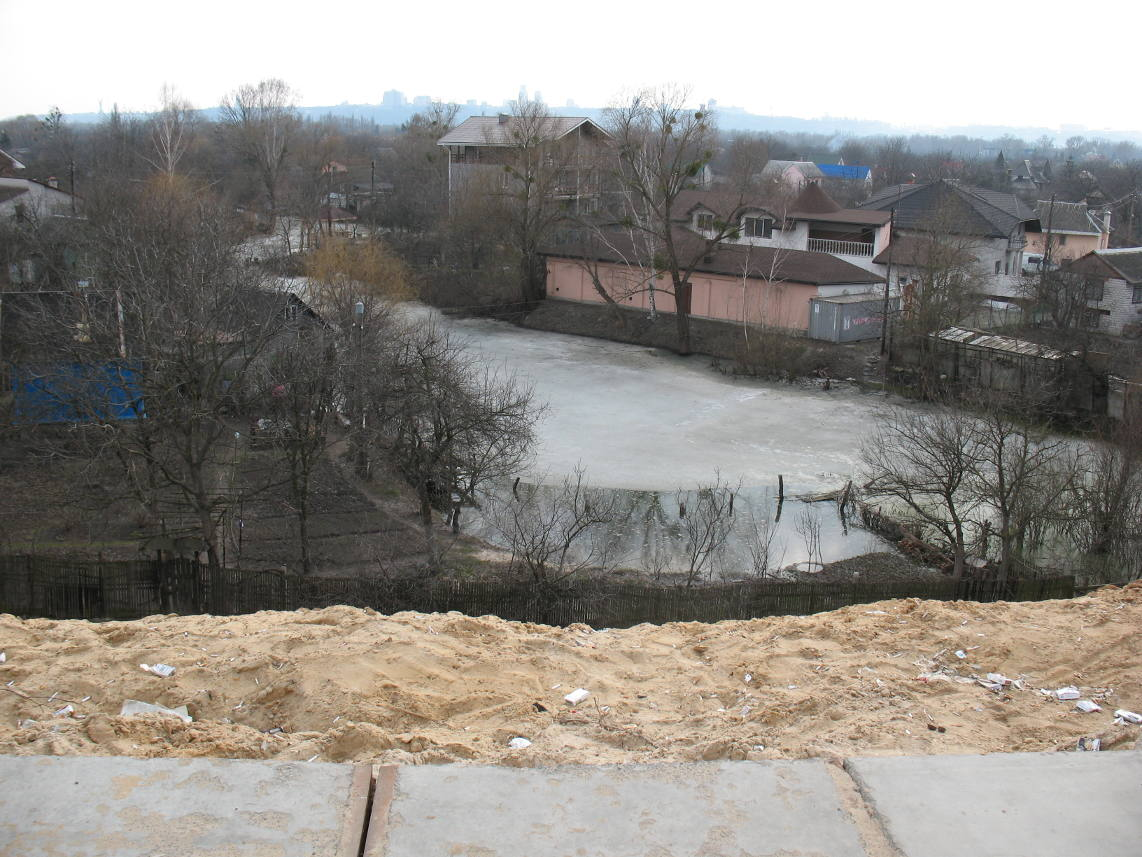
\includegraphics[width=0.98\linewidth]{chast-gorodki/radujnoe/s_IMG_2490.JPG}

\textit{2013 г. Продолжение Малиновки по Русановским садам.}
\end{center}

\newpage

\begin{center}
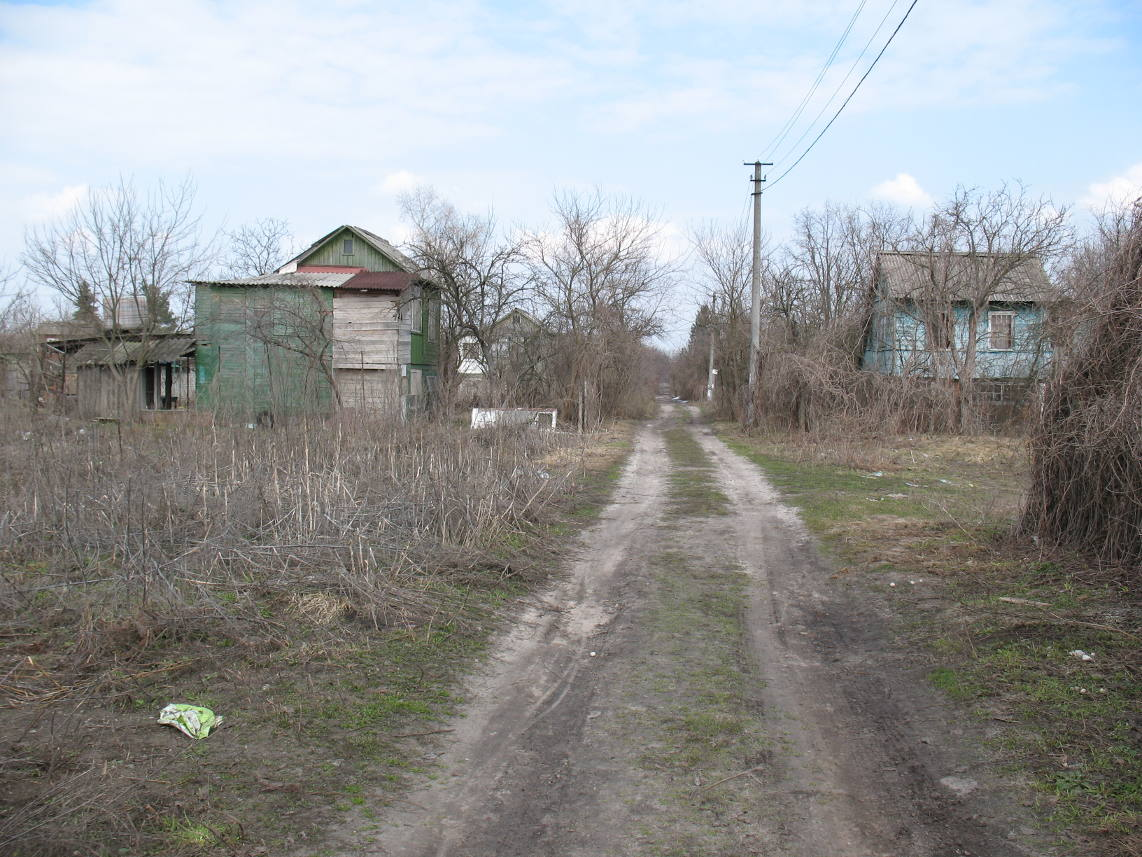
\includegraphics[width=\linewidth]{chast-gorodki/radujnoe/s_IMG_2485.JPG}

\textit{Старый уголок Русановских садов. 2013 год.}
\end{center}

Остался в Русановских садах след не только русла, что продолжало Неводное, но и продолжение Малиновки. Ее тоже перерубила дамба, и длинный отрезанный хвост прослеживается южнее железнодорожной платформы Троещина-2, от 30-й линии по 14-ю, наискось через добрую половину Садов. К Центральной Садовой русло примыкает в районе линий 20, 21, 22.

Озеро Радунка лежит оттуда в шестиста с кепкой метрах на северо-восток, за Садами, дамбой с железной дорогой, да частным сектором остатков Воскресенской слободки.

%Болото Корчовня, или Корчовка было между Выгуровщиной и Воскресенской слободкой, эдак промеж нынешней улицей Кибальчича и проспектом Ватутина. Весь район Кибальчич стоит на бывшем болоте. К середине 20 века его основательно подсушили, а дальше и вовсе извели.

Радунку во второй половине 20 века укоротили на севере, и расширили в южной части, выгнув на восток вместо прежнего запада. Не знаю давней глубины озера, но сейчас до трех метров.

Южнее озера, в продолжающейся ложбине, еще в 1990-х годах были еще два озера, последнее из которых, меньшее, достигало перекрестка улицы Радужной с проспектом Алишера Навои. Я застал там в начале 2010-х уже высохшие котловины между частным сектором и шоссе улицы Радужной. Году в 2015 они начали проворно застраиваться многоэтажным жильем.

На карте 1799 года ниже озера Радунки тоже отмечены два озера, одно при селении «хутор Липецкой», а следующее к югу, меньшее – «озеро Очереватое». Оба почти перпендикулярны Радунке, если б она продолжался по их широты. Я не берусь сопоставлять эти озера с теми, что существовали в 1990-х. Насыпи многочисленных дамб, возникших к западу от Воскресенки еще в первой половине 20 века, совершенно исказили сеть здешних водоемов.

Домики восточного берега Радунки были снесены в 1980-1984 годах при сооружении жилмассива Серова, что лежал между улицей Радужной (над берегом озера) и бульваром Перова. Потом массив Серова добавили к Радужному, коим вначале именовался район у северо-западной части озера (высотки, огибаемые улицей Петра Вершигоры). 

Под раздачу сноса попало слободское кладбище в северной части поселка. А когда уничтожили сельскую Воскресенскую церковь (была между домами по адресам ул. Радужная, 17А и 13В), я не знаю. Некоторые источники сообщают, что в 1930-х, однако известно, что она существовала и в сороковых. В тридцатых же, после закрытия Лавры это была одна из немногих действующих в Киеве и окрестностях церквей.

Застройка западного берега озера Радунки началась после войны, а прежде заселение коснулось лишь восточной стороны озера. Прямо вдоль восточного берега шла улица Шевченковская. Параллельно ей, по слободке – Родонковская (Радонковская) с площадью, где стояла церковь. Север ограничивался Оболонским переулком. Родонковская продолжалась Боярской, пересекаемой Броварским переулком.

Вероятно существует связь между улицей, урочищем Боярским и упоминаемым в документах 17 века островом Богарским, принадлежащим городу, магистрату. На немецкой карте 1943 года показано также болото Боярское, к западу от Малиновки, достигая Черторыи. Теперь там основная часть Воскресенских садов. 

Но больше меня занимает Родонковская улица. Очевидно, это историческое название, связанное с именем озера у слободки. В отличие от современной улицы Радунской на жилмассиве Троещина и Радосыньской в селе Троещине – то именования «ученые».

«Родонковская» же именем восходит одновременно к известной по старинным, с 16 века документам, речке Радунке, но и к летописной Родуни. Какой-то смутный вывод напрашивается от названия сельской улицы, важный и ускользающий от меня.

%А ниже болота Боярского, к югу от железной дороги, было другое болото, Михайловщина, обтекаемая руслом, что слывет ныне Русановским озером.


\begin{center}
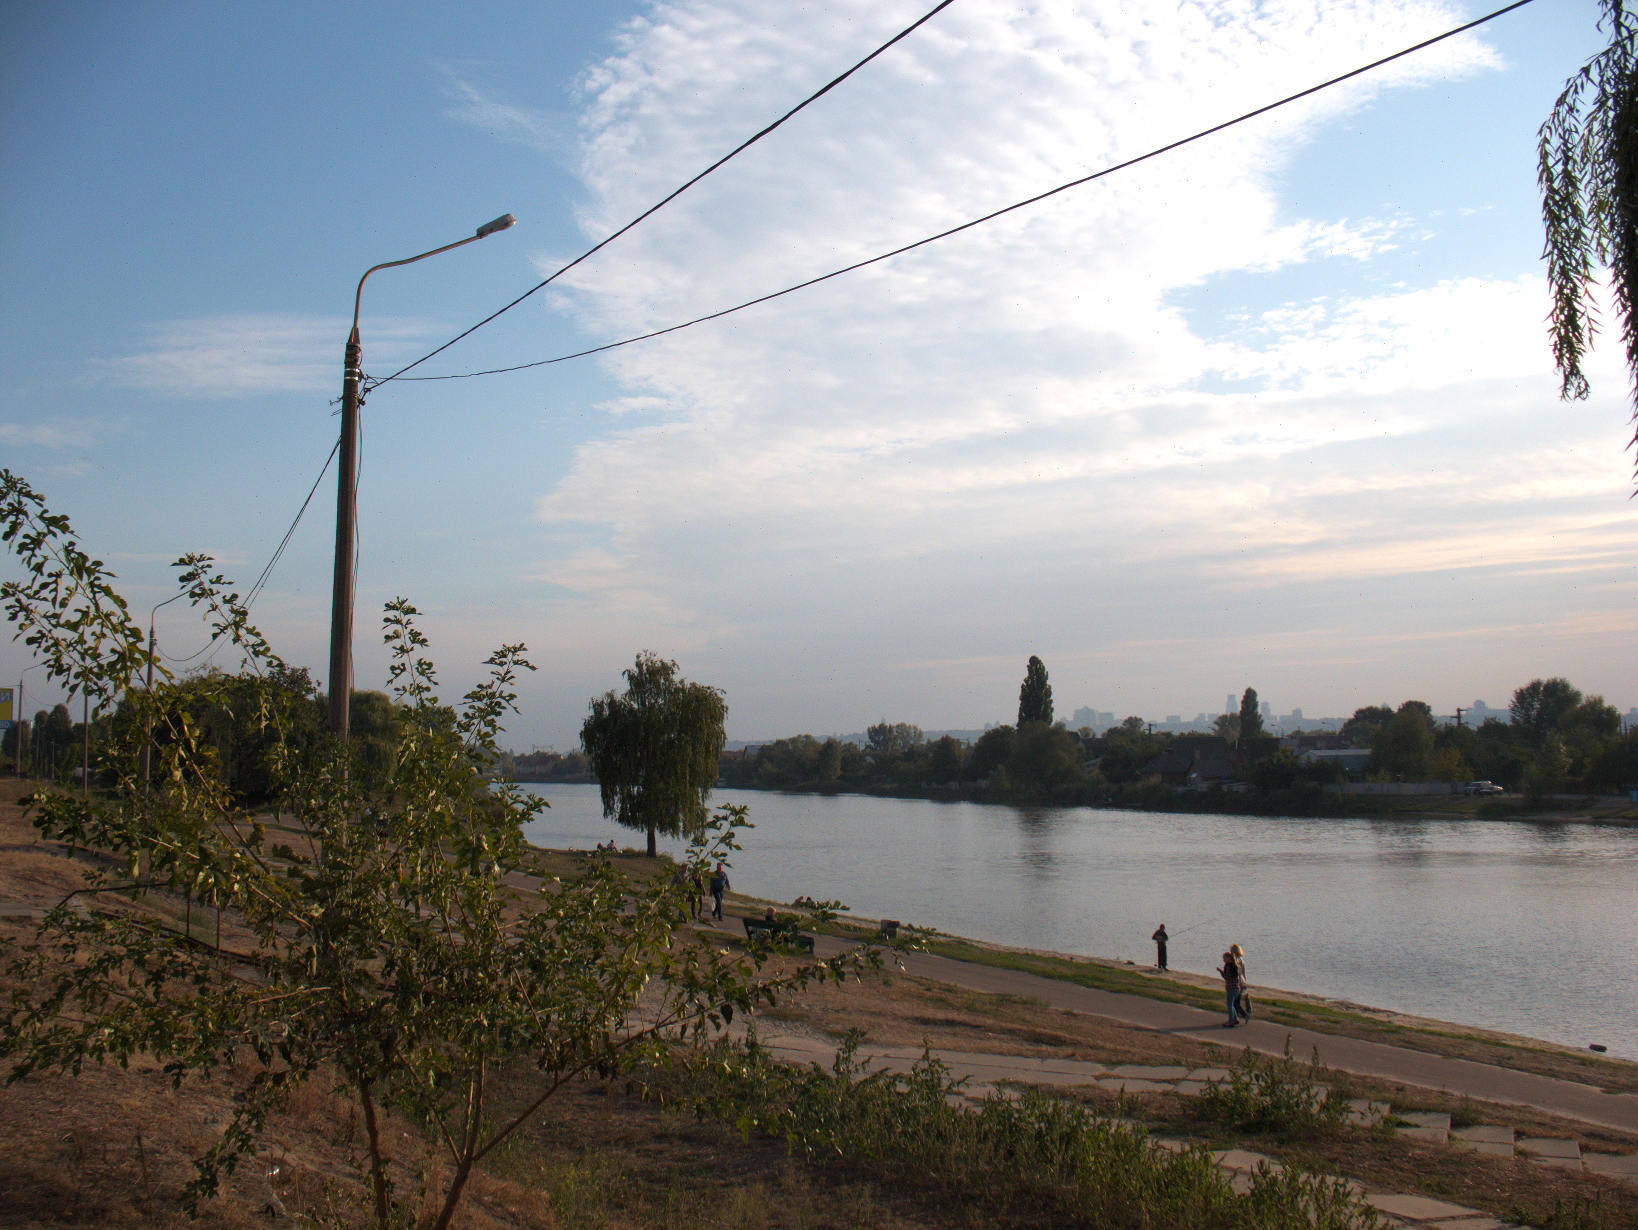
\includegraphics[width=\linewidth]{chast-gorodki/radujnoe/s_raduj-CRW_4036.jpg}

\textit{Озеро Радунка в 2014.}
\end{center}


Как выглядело озеро Радунка раньше, допустим в 1970-е? Желающие могут найти снимки в сети. Например, у южной оконечности озера был хвостик, направленный к улице Марка Черемшины. Радунку перегораживало несколько поросших травой гатей. Зеленая травка покрывала и берега. Из-за заборов на воду выглядывали частные дома. По месту нынешнего мостика через озеро, мостик был и раньше, только узенький, пешеходный. С берега на берег по деревянным столбами перекинулась линия электропередач.

Тогда озеро было еще более, чем сейчас, похоже на тихую равнинную реку.

На 2017 год южный конец его упирается в дорогу, потом продолжается – вдоль улицы Радужной – сухая низина русла, вовсю застраивающаяся. Затем русло уходит в гаражные кооперативы за перекресток Старосельской и Черемшины, и там уж я не ходил дальше. Хотя ложбина существует поныне, на картах со времен Шуберта заполненное водой озеро Радунка имеет почти те же пределы, что сегодня. Цельность русла, с водой или без, говорит о том, что некогда тут протекала река шириной по меньшей мере 100 метров. Имя ее, полагаю, созвучно озеру.

%Я застал ее еще в виде пустырей и лугов между улицей и частным сектором слободки (по улицам Черемшины). 

У западного берега Радунки возвышается и левобережная Лысая гора, только заметить ее мешают дома.
